3D-SCNN modeļa prognozes ar ToF sensoriem iegūtajos ierakstos attēlotas \ref{fig:3dscnn_preds}. attēlā (a). Testa transportlīdzeklim atrodoties ainas vidū, redzams, ka izkliedētā sensoru sistēma spēja uztvert 360 grādu skatu un objektu detektēšanas modelis spēja atšķirt gājējus transportlīdzekļu aklajās zonās. Ieejas temporālā vokseļu kodēšana veikta ar ainas robežām \qtyrange{0}{50}{\metre} $X$ asij, \qtyrange{-25}{25}{\metre} $Y$ asij un \qtyrange{-2}{1}{\metre} $Z$ asij. Optimālajiem vokselizācijas izmēriem \([VS_x, VS_y, VS_z]\) vērtības \(VS_x\), \(VS_y\) un \(VS_z\) iestatītas attiecīgi uz \qty{0.12}{\metre}, \qty{0.12}{\metre} un \qty{0.6}{\metre}. \(VS_z\) vienādi sadala telpu 5 BEV šķēlumos, savukārt divi kanāli \(C\) katrā šķēlumā saglabā detalizētas pazīmes, nepalielinot laika soļu skaitu. Konsekventam salīdzinājumam tie paši parametri izmantoti \textit{KITTI}, \textit{Pandaset} un iegūtajai ToF validācijas datu kopai. Tā kā modelis sākotnēji apmācīts ar LiDAR datu kopām, šie vokselizācijas parametri izvēlēti atbilstoši LiDAR darbības attālumam, vienlaikus saglabājot piemērotību ToF datiem ar īsāku attālumu. \ref{fig:3dscnn_preds}. attēlā (b) parādīts apmācībā izmantotās \textit{Pandaset} uz priekšu vērstā LiDAR datu kopas punktu mākonis un prognozētie objektu ietverošie paralēlskaldņi.

Iegūtā ToF datu kopa manuāli marķēta automobiļu, gājēju un velosipēdistu objektu klasēm. Atšķirībā no \textit{KITTI} etalontesta marķējumi neietvēra grūtības līmeņu klasifikāciju. Tādēļ detektēšanas veiktspēja ToF datu kopā novērtēta bez sadalījuma vieglajā, vidējā un sarežģītajā kategorijā. Atbilstībai \textit{KITTI} novērtēšanas protokolam norādītie rezultāti izmanto automobiļu klases \Gls{bev} \Gls{ap} ar \Gls{iou} slieksni 0,7.

\begin{figure}[!t]
\centering
\begin{subfigure}{0.49\textwidth}
    \centering
    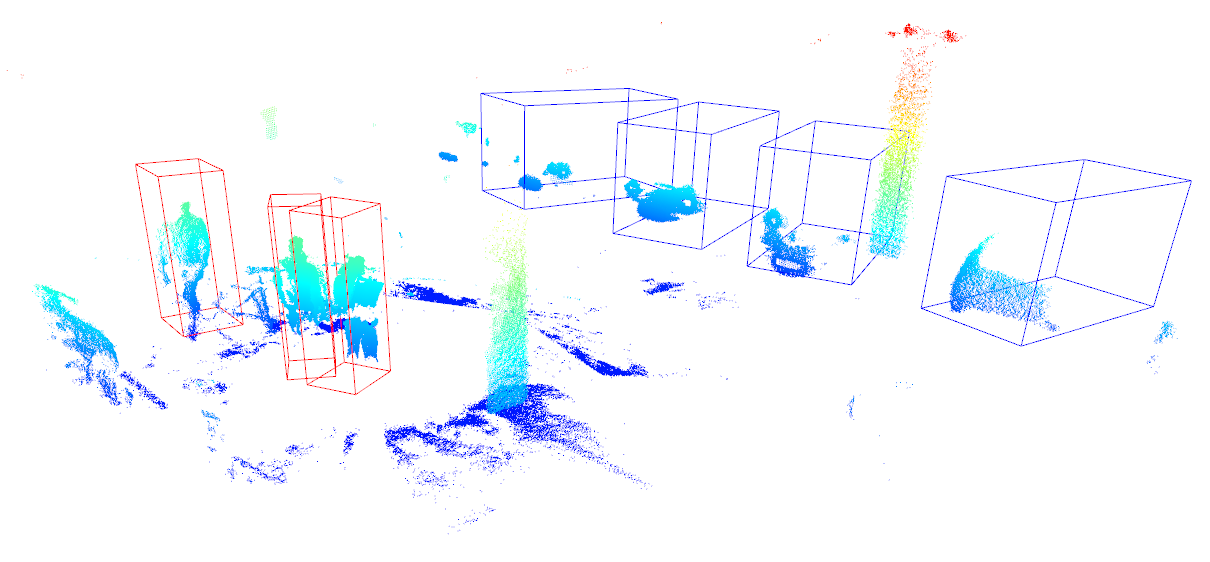
\includegraphics[width=\linewidth]{fig/snn_alfa_detections.png}
    \captionsetup{justification=centering}
    \caption{}
    \label{fig:3dscnn_pred_alfa}
\end{subfigure}
\hfill
\begin{subfigure}{0.49\textwidth}
    \centering
    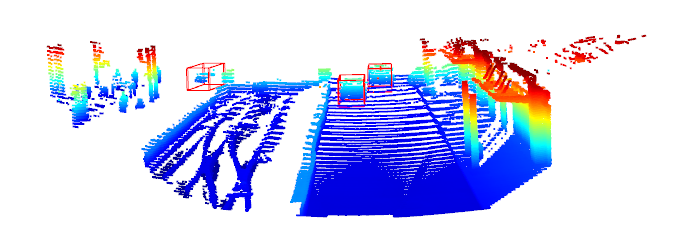
\includegraphics[width=\linewidth]{fig/snn_panda_detections.png}
    \captionsetup{justification=centering}
    \caption{}
    \label{fig:3dscnn_pred_panda}
\end{subfigure}
\caption{3D-SCNN objektu prognozes: (\textbf{a}) ToF datos, kas iegūti, apvienojot vairāku sensoru datus; (\textbf{b}) Pandaset neskenējošā LiDAR datu kopas ainā.}
\label{fig:3dscnn_preds}
\end{figure}

Modeļu apmācības rezultāti dažādās datu kopās apkopoti \ref{table:snn_map}. tabulā. Salīdzināšanai \textit{VGG-11} un \textit{VGG-13} modeļi atsevišķi apmācīti ar \textit{KITTI} un \textit{Pandaset}, pēc tam novērtēti gan attiecīgajās apmācības datu kopās, gan iegūtajos ToF datos. Mērķis bija izvērtēt to vispārināšanas spēju starp dažādām sensoru modalitātēm. Papildus modeļi salīdzināti ar modernākajiem uz LiDAR balstītajiem \Gls{snn} uztveres modeļiem \cite{Zhou2020, qiu2024}. Ar \textit{KITTI} apmācītie modeļi uzrādīja labus rezultātus pašā \textit{KITTI} datu kopā: \textit{VGG-13} sasniedza augstāku AP (75,3~\%) nekā \textit{VGG-11} (70,7~\%). Tomēr, pārbaudot tos ToF datos, novērots būtisks veiktspējas kritums, īpaši \textit{VGG-11} gadījumā (40,0~\% \textit{VGG-11} un 65,0~\% \textit{VGG-13}), uzsverot domēnu atšķirību starp LiDAR balstītajiem \textit{KITTI} datiem un ToF punktu mākoņiem. Tas liecina, ka modeļiem, kas apmācīti tikai ar LiDAR datiem, ir grūti pielāgoties ToF signālu īpašībām. Savukārt ar \textit{Pandaset} apmācītie modeļi demonstrēja vienmērīgāku veiktspēju dažādās datu kopās. Ar \textit{Pandaset} apmācītie \textit{VGG-11} un \textit{VGG-13} sasniedza attiecīgi 69,0~\% un 71,0~\% AP \textit{Pandaset} datos. Būtiski, ka apmācība ar \textit{Pandaset} uzlaboja \textit{VGG-11} ToF detektēšanas veiktspēju un nodrošināja labāku pārnesamību uz ToF datiem — 55,0~\% AP. Savukārt ar \textit{KITTI} apmācītais \textit{VGG-13} sasniedza augstāko ToF AP — 65,0~\%. Šie rezultāti liecina, ka \textit{Pandaset} uz priekšu vērstā neskenējošā LiDAR lielāka līdzība ar ToF uztveri nekā \textit{KITTI} 360 grādu LiDAR var uzlabot pārnesamību un apmācības precizitāti, taču vispārināšana starp modalitātēm var būt atkarīga gan no apmācības datu kopas, gan tīkla arhitektūras, kā \textit{VGG-13} gadījumā.

\begin{table}[ht]
\centering
\caption{Modeļu parametru, retinājuma un automobiļu klases BEV AP salīdzinājums dažādās datu kopās}
\label{table:snn_map}
\footnotesize

\setlength{\tabcolsep}{3pt}
\begin{adjustbox}{max width=\textwidth}\begin{tabular}{l c c c c c}
\toprule
\textbf{Modelis} & \textbf{Datu kopa} & \textbf{Ieeja} & \textbf{Param. sk. (M)} & \textbf{Retinājums (\%)} & \textbf{AP (\%)} \\
\midrule
\textbf{Saistītie darbi---SNN}  & & & & & \\
  Zhou u.\,c. SNN \cite{Zhou2020}  & KITTI & Vokselis & - & - & 67{,}00 \\
  Zhou u.\,c. SNN ar SC \cite{Zhou2020}  & KITTI & Vokselis & - & - & 68{,}27 \\
\midrule
\textbf{Saistītie darbi---ANN}  & & & & & \\
  PointPillar \cite{lang2019} & KITTI & Stabs & 18 & - & 86{,}48 \\
  PV-RCNN \cite{shi2020} & KITTI & PV & 50 & - & 90{,}59 \\
\midrule
\textbf{Šis darbs---SNN}  & & & & & \\
\multirow{2}{*}{\raggedright SVGG-11  (Apmācīts ar KITTI)}
    & KITTI & TVC & 12{,}8 & 55{,}73 & 70{,}7  \\
    & ToF   & TVC & 12{,}8 & 35{,}10 & 40{,}0  \\
\midrule
\multirow{2}{*}{\raggedright SVGG-13  (Apmācīts ar KITTI)}
    & KITTI & TVC & 13{,}1 &  63{,}67 & 75{,}3  \\
    & ToF   & TVC & 13{,}1 &  45{,}05 & 65{,}0  \\
\midrule
\multirow{2}{*}{\raggedright SVGG-11  (Apmācīts ar Pandaset)}
    & Pandaset & TVC & 12{,}8 & 50{,}26 & 69{,}0 \\
    & ToF      & TVC & 12{,}8 & 20{,}15 & 55{,}0 \\
\midrule
\multirow{2}{*}{\raggedright SVGG-13  (Apmācīts ar Pandaset)}
    & Pandaset & TVC & 13{,}1 & 42{,}15 & 71{,}0 \\
    & ToF      & TVC & 13{,}1 & 32{,}67 & 60{,}0 \\
\bottomrule
\end{tabular}\end{adjustbox}

\end{table}


